\documentclass{beamer}
\usepackage[utf8]{inputenc}
\usepackage[spanish]{babel}
\usetheme{metropolis}           % Use metropolis theme
\graphicspath{{images/}}

\usepackage{multirow}
\usepackage{multicol}
\usepackage{graphicx}
\usepackage{listings}
\usepackage[default]{sourcesanspro}

\usepackage[scale=2]{ccicons}

\usepackage[
    type={CC},
    modifier={by-nc-sa},
    version={4.0},
]{doclicense}



\hypersetup{
    colorlinks=true,
    linkcolor=black,
    filecolor=magenta,
    urlcolor=cyan,
}

\title{Diseño de un sistema basado en reglas para la estimación de la edad a partir de los huesos del pubis mediante machine learning explicable.}

\date{12 de julio de 2022}
\author{\small Autor: Antonio David Villegas Yeguas (\textit{advy99@correo.ugr.es}) \\ Directores: Óscar Cordón García y Sergio Damas Arroyo}
\institute[UGR]{

\includegraphics[scale = 0.075]{ugr.png} \quad 
\includegraphics[scale = 0.075]{logo_etsiit.png} \quad 
\includegraphics[scale = 0.175]{posgrado.jpg}\\
\doclicenseThis
}
\setbeamertemplate{caption}{\raggedright\insertcaption\par}

\begin{document}

 \maketitle

\begin{frame}{Índice}
\tableofcontents
\end{frame}




\section{Objetivos del trabajo e introducción al problema}
\begin{frame}{Objetivos}
Los objetivos de este trabajo se centran en:

\begin{enumerate}
	\item Categorizar el problema y estudiar los trabajos anteriores.
	\item Analizar los datos disponibles.
	\item Estudiar algoritmos evolutivos para inferir reglas.
	\item Implementar un sistema basado en reglas capaz de resolver el problema.
	\item Analizar y estudiar los resultados.
\end{enumerate}

\end{frame}

\begin{frame}{Estimación de la edad a partir de los huesos del pubis}

	\begin{columns}[T]
		\begin{column}{.4\textwidth}
			\begin{itemize}
				\item Problema real de gran interés.
				\item Problema complejo.
				\item No existe un método concreto.
				\item Trabajo subjetivo por parte de forenses.
				\item Falta de muestras para edades tempranas.
				\item Primera propuesta por T. W. Todd en 1920.
			\end{itemize}

		\end{column}

		\begin{column}{.7\textwidth}
			\begin{table}[H]
				\centering
				\resizebox{1\textwidth}{!}{%
					\begin{tabular}{|c|c|c|}
					\hline
					Crestas y surcos: Muy definidos & Superficie porosa irregular: Sí & Borde superior: Definido  \\ \hline
					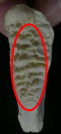
\includegraphics[scale = 0.75]{huesos/crestas_surcos_muy_definidos.png}  &   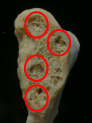
\includegraphics[scale = 0.75]{huesos/superficie_porosa_si.png} &  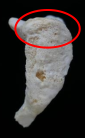
\includegraphics[scale = 0.75]{huesos/borde_superior_definido.png}  \\ \hline
					Nódulo óseo: Presente & Borde inferior: No definido & Borde dorsal: Definido \\ \hline
					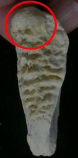
\includegraphics[scale = 0.75]{huesos/nodulo_oseo_presente.png} & 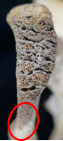
\includegraphics[scale = 0.75]{huesos/borde_inferior_no_definido.png} &  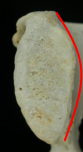
\includegraphics[scale = 0.75]{huesos/borde_dorsal_definido.png} \\ \hline
					Plataforma dorsal: Presente & Bisel ventral: En proceso de formación & Borde ventral: Muchas excrecencias \\ \hline
					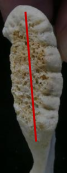
\includegraphics[scale = 0.75]{huesos/plataforma_dorsal_presente.png} & 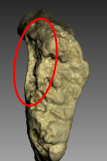
\includegraphics[scale = 0.75]{huesos/bisel_ventral_en_proceso_formacion.png} &   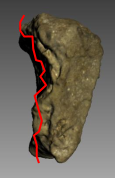
\includegraphics[scale = 0.75]{huesos/borde_ventral_muchas_excrecencias.png} \\ \hline
					\end{tabular}%
				}
				\caption{Algunos ejemplos de las características consideradas por Todd.}\label{table:caracteristicas_todd}
			\end{table}
		\end{column}

	\end{columns}


\end{frame}


\section{Estado del arte}
\begin{frame}[allowframebreaks]{Estado del arte}

\begin{itemize}
\item 1953 a 1973: Gilbert y McKern. Cambio de enfoque a regresión.

\item 1990: J. M. Suchey y S. Brooks. Reducción del número de fases.

\item 2015: D. E. Slice y Algee-Hewitt. Escaneo de huesos utilizando Visión por Computador, utilizando 41 muestras.

\item 2018: A. Kotěrová, D. Navega, M. Štepanovský, Z. Buk, J. Brůžek y E. Cunha. Distintos modelos de aprendizaje, y un conjunto de datos más significativo, de 941 muestras.

\item 2022: J. C. Gámez-Granados, J. Irurita, R. Pérez, A. González, S. Damas, I. Alemán y O. Cordón (sometido a revista). Aprendizaje de reglas de forma iterativa.

\end{itemize}

\end{frame}


\section{Inteligencia Artificial Explicable}
\begin{frame}{Inteligencia Artificial Explicable}

	Producir modelos fácilmente interpretables manteniendo buenos resultados y permitir que sean transparentes de cara a entender su funcionamiento.

	\begin{figure}[H]
		\centering
		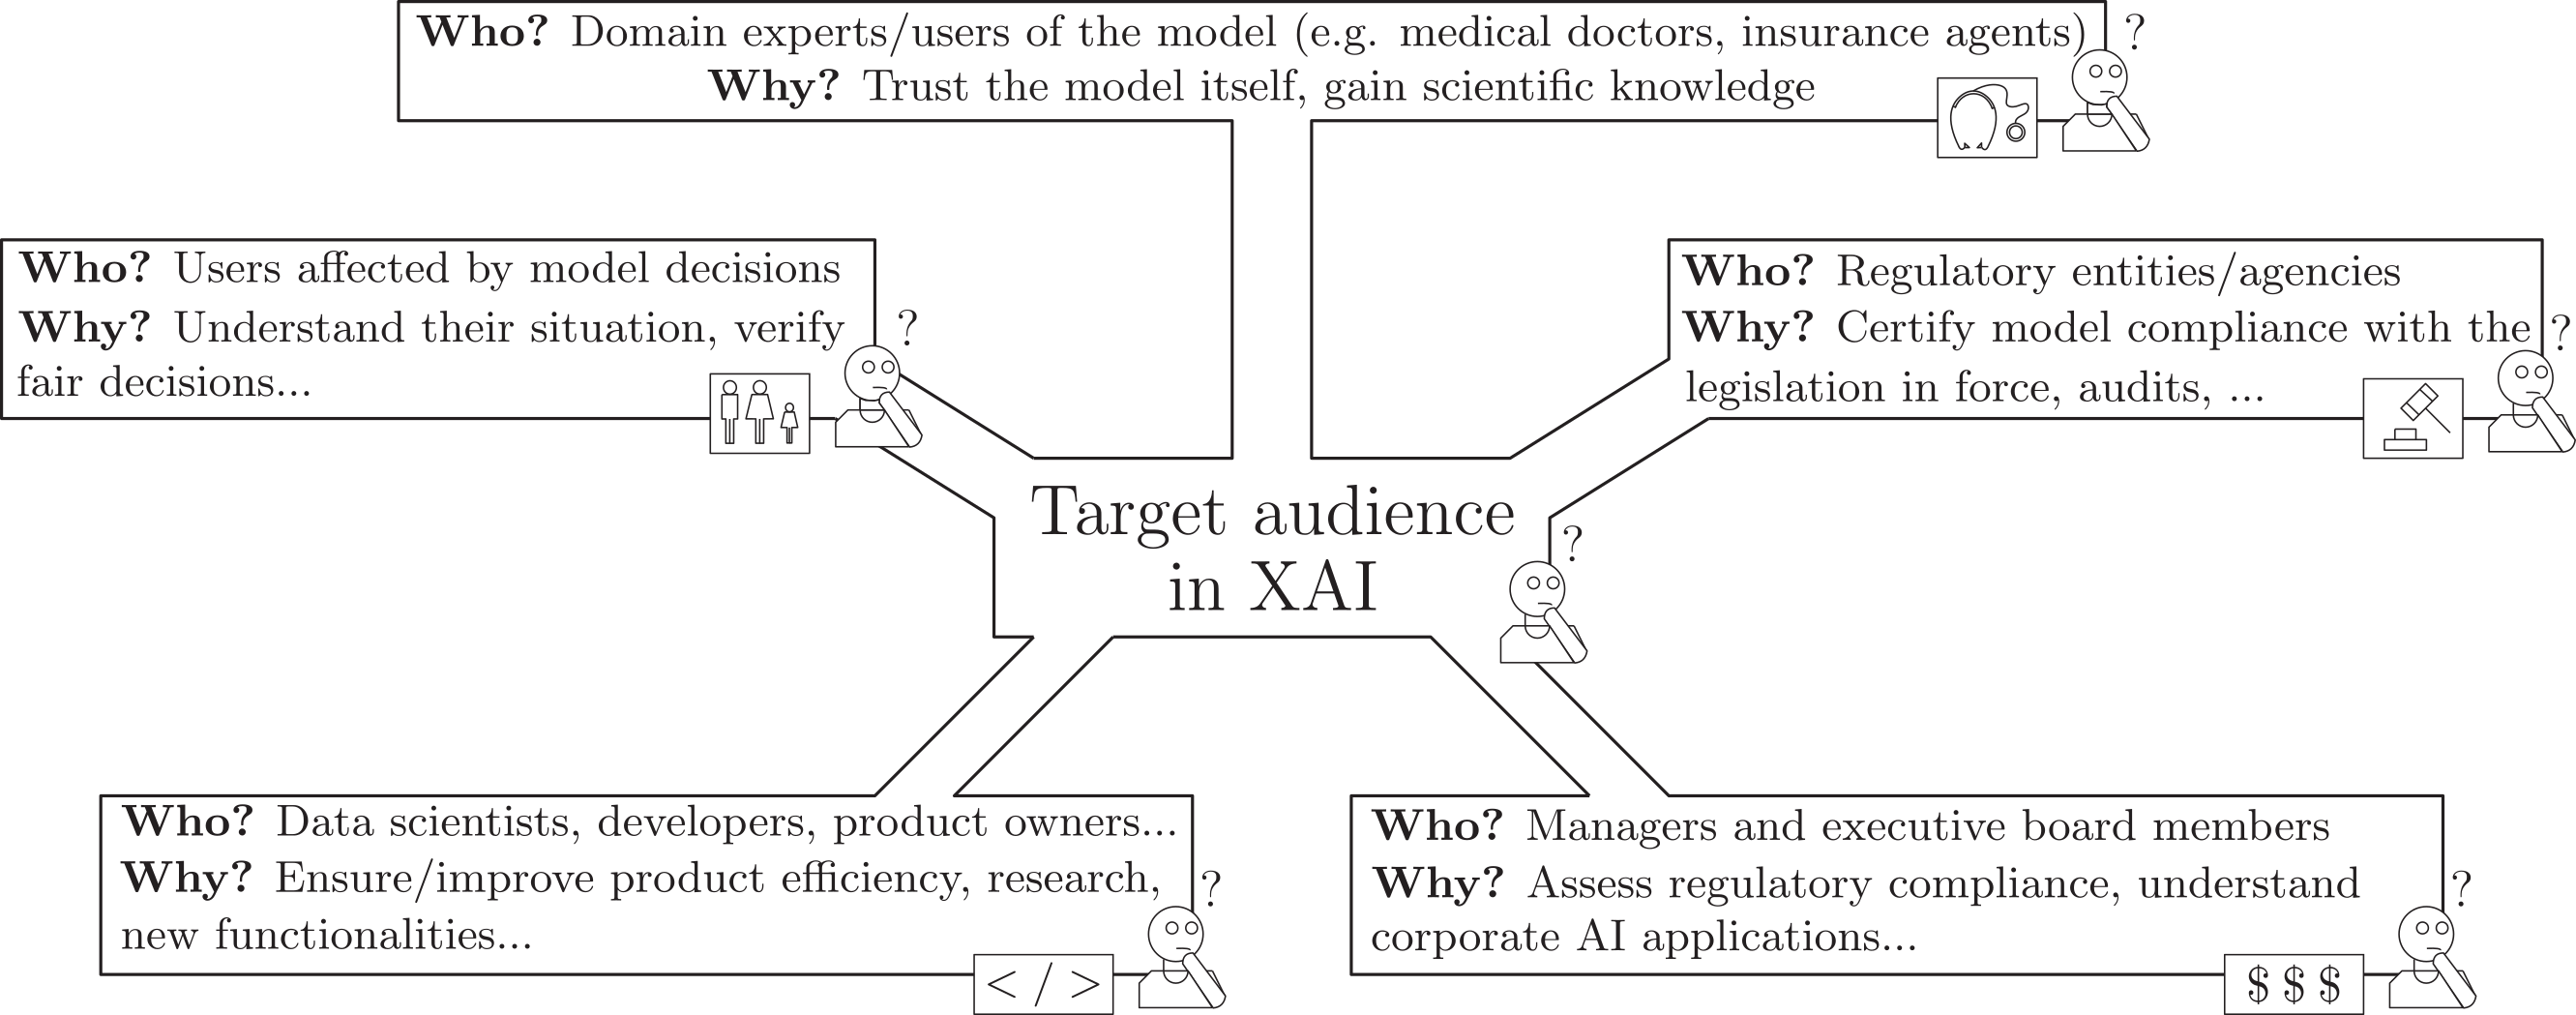
\includegraphics[scale = 0.65]{esquema_xai.png}
		\caption{Diagrama de las ventajas de la Inteligencia Artificial Explicable desde varios puntos de vista.}
		\label{fig:esquema_xai}
	\end{figure}

\end{frame}

\section{Propuesta de trabajo y entorno experimental}
\begin{frame}{Conjunto de datos}
	Principales características:

	\begin{enumerate}
		\item 960 muestras: 473 de la lateralidad izquierda y 487 de la lateralidad derecha.
		\item 9 atributos categóricos.
		\item 10 rangos de edad (atributo a predecir). Problema de clasificación ordinal.
		\item Rango de edades: 18 a 82 años.
		\item Clasificadas manualmente por el Laboratorio de Antropología Física de la UGR.
		\item Altamente desbalanceado.
	\end{enumerate}
\end{frame}


\begin{frame}{Conjunto de datos}

	\begin{figure}[H]
		\centering
		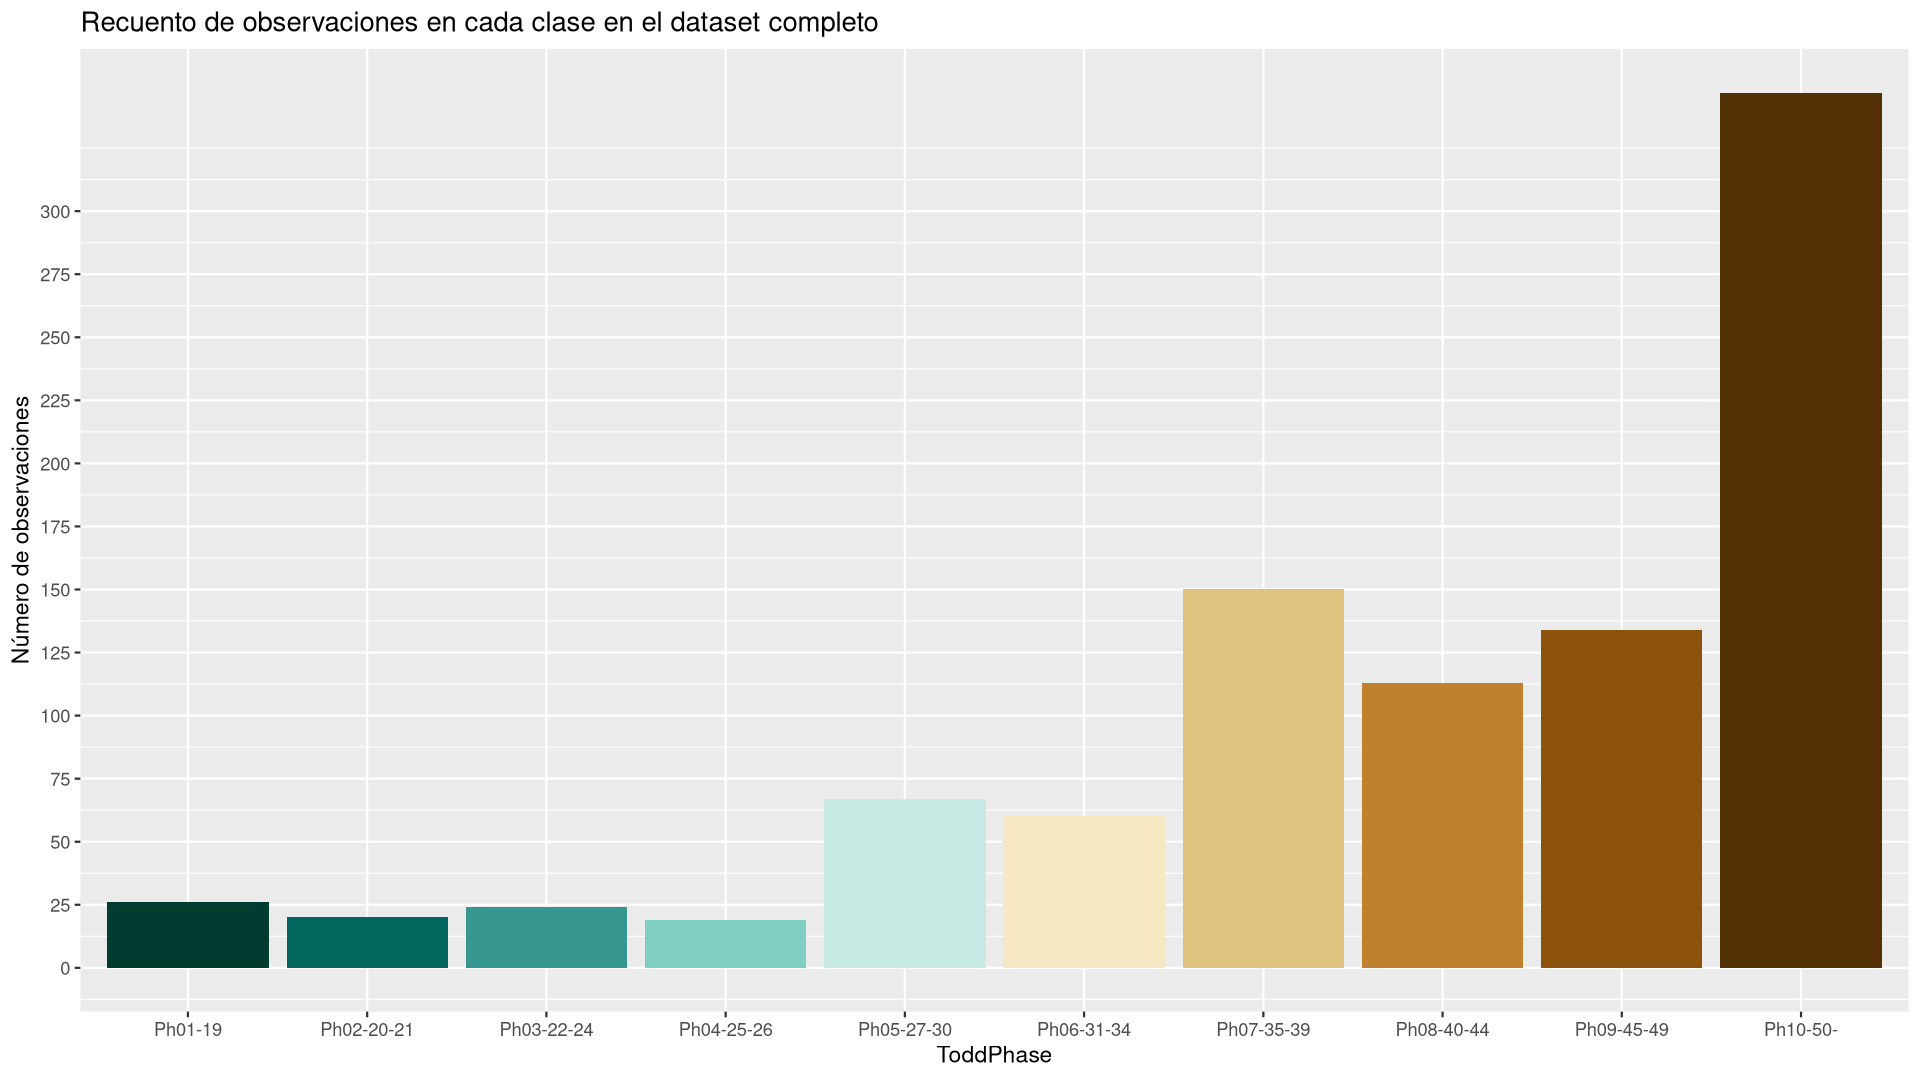
\includegraphics[width=\textwidth]{distribucion_clases_completo.png}
		\caption{Distribución de las observaciones según su clase.}
		\label{fig:distribucion_clases_completo}
	\end{figure}

\end{frame}


\begin{frame}{Enfoque utilizado}

	\begin{itemize}
		\item Enfoque propuesto por Todd. Clasificación en diez clases.
		\item Clasificación usando un conjunto de reglas.
		\item Programación Genética para aprender expresiones.
		\item Selección de características por parte del modelo.
		\item Validación de los resultados con un conjunto de test del 20\% de los datos y validación cruzada de 5 folds en entrenamiento.
		\item Sobremuestreo de datos sobre el conjunto de entrenamiento, utilizando sobremuestreo aleatorio, SMOTE y BorderlineSMOTE.
	\end{itemize}

\end{frame}

\begin{frame}{Preprocesado: Sobremuestreo de datos con ROS}
	Sobremuestreo aleatorio:
	\begin{itemize}
		\item Se basa en duplicar observaciones ya existentes en el conjunto de datos.
		\item No introduce observaciones sintéticas.
	\end{itemize}
\end{frame}

\begin{frame}{Preprocesado: Sobremuestreo de datos con SMOTE}

	\begin{columns}[T]
		\begin{column}{.5\textwidth}
			Sobremuestreo con SMOTE:

			\begin{itemize}
				\item Propuesto en 2002.
				\item Uso de la variante SMOTEN, para datos categóricos.
			\end{itemize}

			\vspace{1cm}

			Sobremuestreo con BorderlineSMOTE:

			\begin{itemize}
				\item Modificación de SMOTE propuesta en 2005.
				\item Uso de observaciones frontera.
			\end{itemize}

		\end{column}

		\begin{column}{.5\textwidth}
			\vspace*{-0.5cm}
			\begin{figure}[H]
			    \centering
				 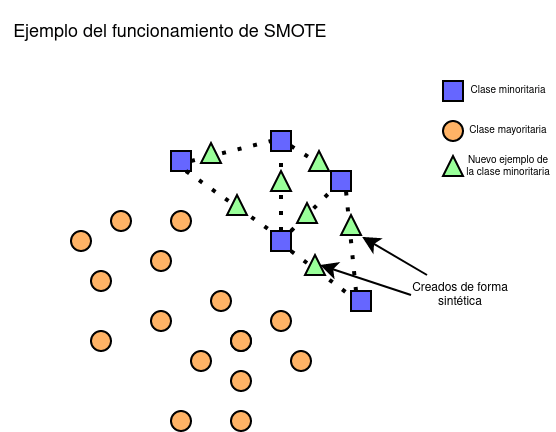
\includegraphics[width=0.75\textwidth]{funcionamiento_smote.png}
			    \caption{Funcionamiento de SMOTE.}
				 \label{fig:funcionamiento_smote}
			\end{figure}

			\vspace*{-0.75cm}
			\begin{figure}[H]
				 \centering
				 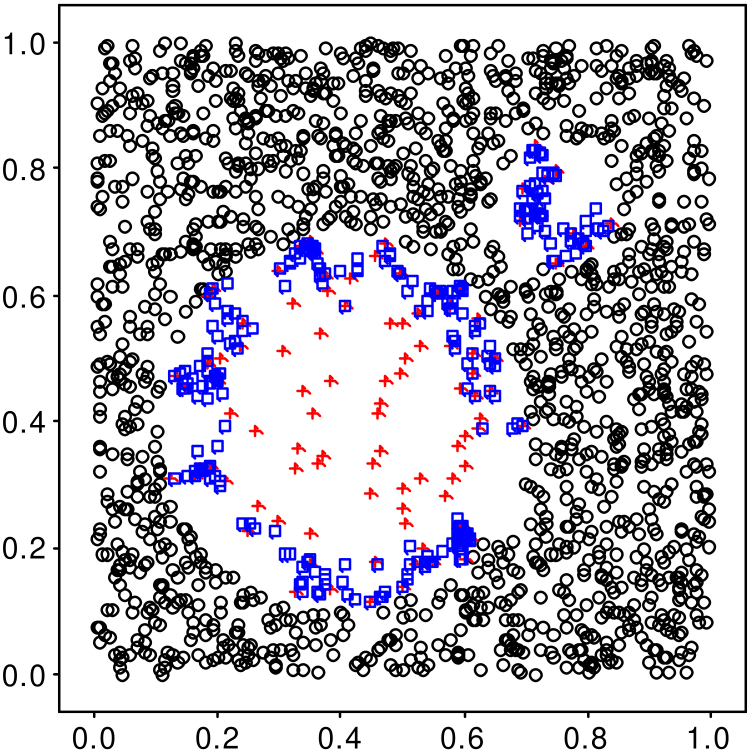
\includegraphics[width=0.6\textwidth]{bl-smote-datos-sinteticos.png}
				 \caption{Funcionamiento de BL-SMOTE.}
				 \label{fig:bl-smote-datos-sinteticos}
			\end{figure}
		\end{column}

	\end{columns}

\end{frame}



\begin{frame}{Algoritmos: Programación Genética}

	\begin{columns}[T]

		\begin{column}{.4\textwidth}
			\begin{itemize}
				\item Propuesto por John Koza en 1990.
				\item Algoritmo evolutivo.
				\item Uso de árboles en lugar de cromosomas.
				\item Distintos tipos de problemas.
				\item Resultado: Árbol que mejor se ajusta a los datos.
				\item En nuestro caso, los árboles representan reglas de clasificación.
			\end{itemize}
		\end{column}


		\begin{column}{.6\textwidth}
			\begin{figure}[H]
			    \centering
				 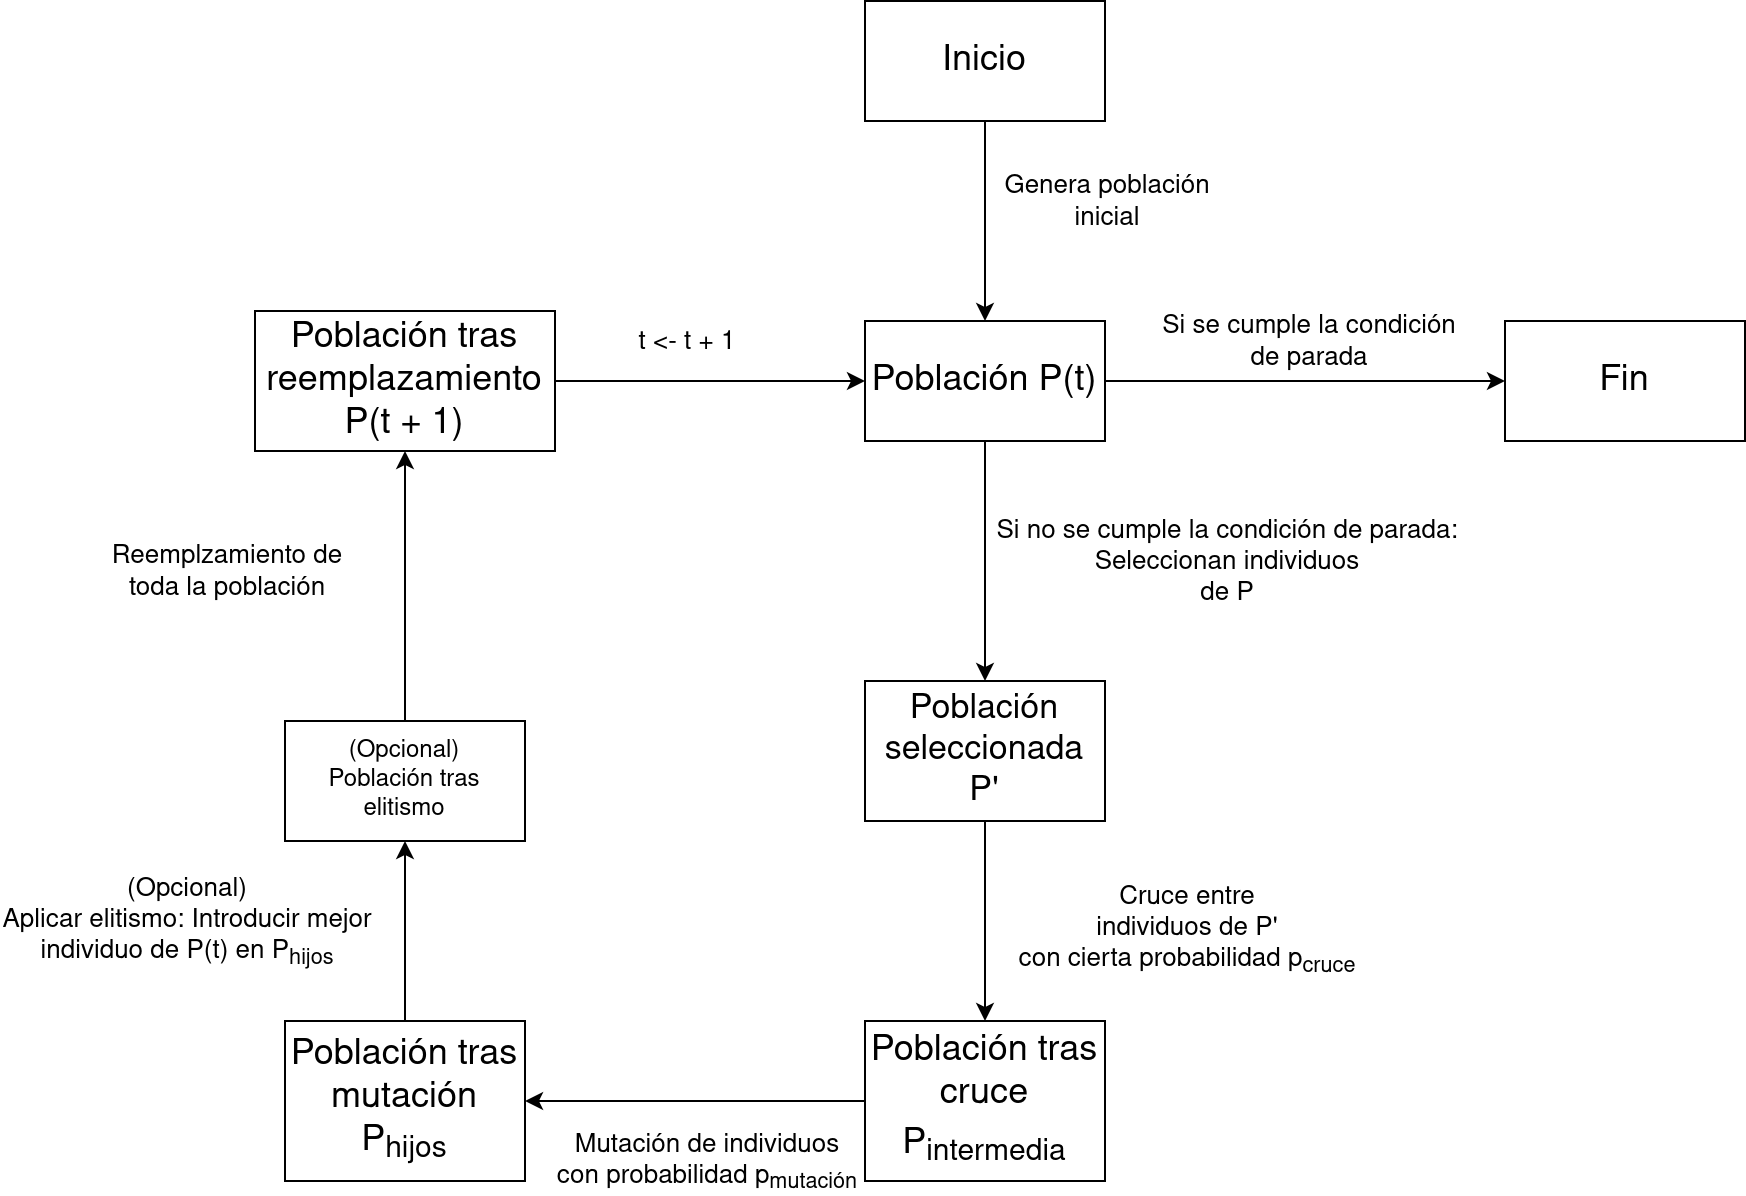
\includegraphics[width=\textwidth]{generacional.png}
			    \caption{Esquema de un algoritmo evolutivo con un modelo generacional.}
				 \label{fig:modelo_generacioal}
			\end{figure}
		\end{column}

	\end{columns}

\end{frame}

\begin{frame}{Algoritmos: Programación Genética para aprender reglas}
	\textbf{El requisito de clausura}: La salida de un nodo ha de poder ser usada como entrada de cualquier nodo padre dentro del árbol. Evita la construcción de árboles erróneos.

	Posibles soluciones:

	\begin{itemize}
		\item Binarizar los símbolos terminales y usar solo funciones booleanas.
		\item Añadir restricciones en los nodos, y tenerlas en cuenta en los operadores de Programación Genética.
		\item Usar un algoritmo de Programación Genética basado en gramáticas.
	\end{itemize}

	En nuestro caso se ha utilizado la última solución.

\end{frame}

\begin{frame}{Algoritmos: Programación Genética para aprender reglas}
	\textbf{Representación de la población}: Un individuo puede ser una regla (clasifica una clase), o bien un conjunto de reglas completo:

	\begin{itemize}
		\item Enfoque Michigan: Un individuo es una regla. Solución parcial al problema. Es necesario lanzar el algoritmo tantas veces como clases tenga el problema.
		\item Enfoque Pittsburgh: Un individuo es un conjunto de reglas, una solución completa al problema. Entrenamiento más complejo y costoso.
	\end{itemize}

\end{frame}

\begin{frame}{Algoritmos: Programación Genética para aprender reglas}
	Utilizaremos tres algoritmos:

	\begin{itemize}
		\item Algoritmo de Falco: Enfoque Michigan. Una solución es una regla, la mejor de la población.
		\item Algoritmo de Tan: Enfoque Michigan. La solución es el conjunto de reglas no repetidas de la población elitista.
		\item Algoritmo de Bojarczuk: Enfoque hibrido, un individuo representa las reglas de un consecuente (una clase concreta).
	\end{itemize}

	Se han \textbf{modificado los algoritmos} para guiar la búsqueda por \textbf{Ordinal Mean Absolute Error (OMAE) como función de fitness}, al ser un problema de clasificación ordinal.

\end{frame}

\begin{frame}{Algoritmos: Validación de los resultados}

	\begin{figure}[H]
		 \centering
		 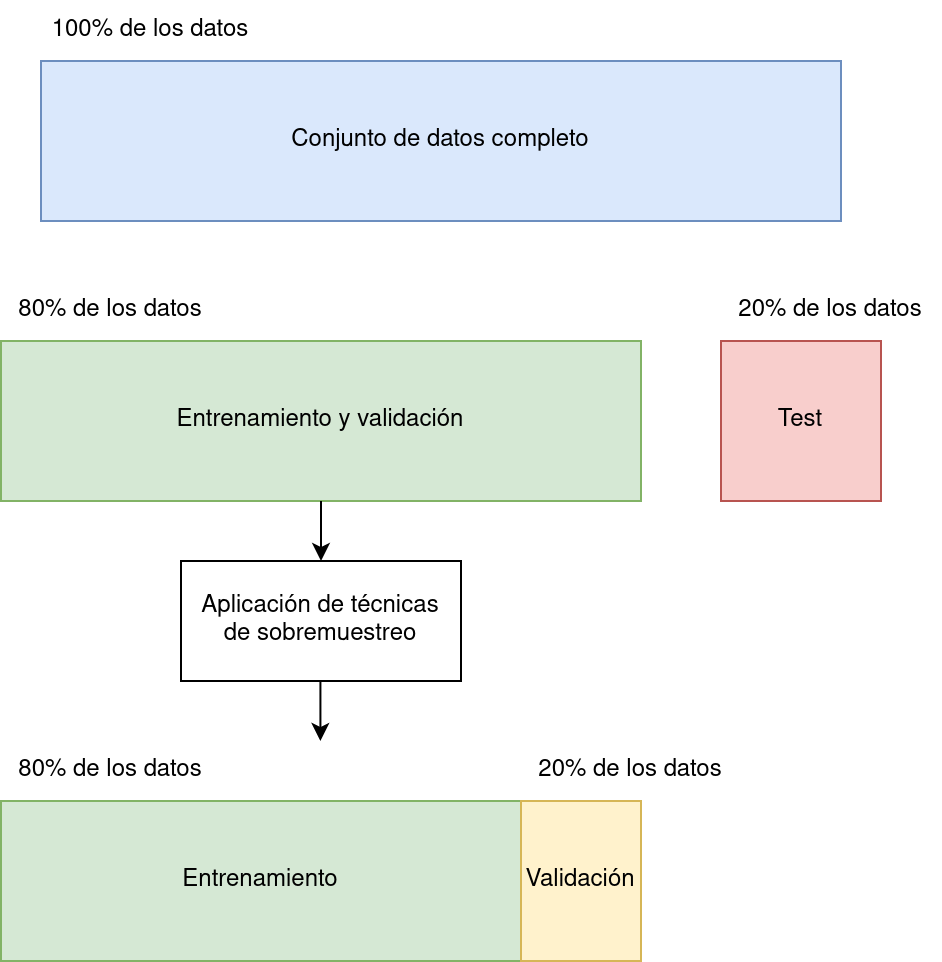
\includegraphics[width=0.6\textwidth]{separacion_train_test.png}
		 \caption{Separación aplicada a los datos.}
		 \label{fig:separacion_train_test}
	\end{figure}

\end{frame}

\begin{frame}{Tecnologías utilizadas}

	% Please add the following required packages to your document preamble:
	% \usepackage{graphicx}
	\begin{table}[H]
	\centering
	\resizebox{\textwidth}{!}{%
	\begin{tabular}{cc}
	
\includegraphics[width=0.10\textwidth]{logos/R.png} & 
\includegraphics[width=0.23\textwidth]{logos/python.png} \\
	
\includegraphics[width=0.15\textwidth]{logos/git.png} & 
\includegraphics[width=0.2\textwidth]{logos/github.png} \\
	\end{tabular}%
	}
	\end{table}
	\begin{figure}[H]
		 \centering
		 
\includegraphics[width=0.25\textwidth]{logos/jclec.png}
	\end{figure}


\end{frame}


\section{Experimentos y análisis de resultados}

\begin{frame}{Experimentos}

	\begin{itemize}
		\item Tres conjuntos de datos: ROS, SMOTE y BorderlineSMOTE.
		\item Tres algoritmos: Tan, Falco y Bojarczuk.
		\item Dos funciones de ajuste para Tan y Falco (propuesta por los algoritmos y OMAE).
		\item Cuatro funciones de ajuste para Bojarczuk (propuesta por el algoritmo, OMAE, AMAE y MMAE).
		\item Ejecuciones con RandomForest y una red neuronal de dos capas totalmente conectadas para comparación de resultados.
	\end{itemize}

\end{frame}

% \begin{frame}{Importancia de la función de ajuste}
%
% 	% Please add the following required packages to your document preamble:
% 	% \usepackage{multirow}
% 	% \usepackage{graphicx}
% 	\begin{table}[H]
% 	\centering
% 	\resizebox{\textwidth}{!}{%
% 	\begin{tabular}{|ccccccc|}
% 	\hline
% 	\multicolumn{7}{|c|}{\textbf{\begin{tabular}[c]{@{}c@{}}Comparación de los resultados del algoritmo de Bojarczuk con \\ sobremuestreo aleatorio y distintas funciones de ajuste.\end{tabular}}}                                                  \\ \hline
% 	\multicolumn{1}{|c|}{\multirow{2}{*}{\textbf{}}} & \multicolumn{3}{c|}{\textbf{OMAE}}                                                                       & \multicolumn{3}{c|}{\textbf{Accuracy}}                                             \\ \cline{2-7}
% 	\multicolumn{1}{|c|}{}                           & \multicolumn{1}{c|}{Training} & \multicolumn{1}{c|}{Validacion} & \multicolumn{1}{c|}{Test}              & \multicolumn{1}{c|}{Training} & \multicolumn{1}{c|}{Validacion} & Test             \\ \hline
% 	\multicolumn{1}{|c|}{\textbf{BJR-ROS-ORIG}}      & \multicolumn{1}{c|}{3,2632} & \multicolumn{1}{c|}{3,2596}    & \multicolumn{1}{c|}{3,2685}          & \multicolumn{1}{c|}{0,1007}  & \multicolumn{1}{c|}{0,1010}    & 0,1573           \\ \hline
% 	\multicolumn{1}{|c|}{\textbf{BJR-ROS-OMAE}}      & \multicolumn{1}{c|}{1,8573} & \multicolumn{1}{c|}{1,9112}   & \multicolumn{1}{c|}{\textbf{1,9691}} & \multicolumn{1}{c|}{0,2216}  & \multicolumn{1}{c|}{0,2080}    & 0,0927          \\ \hline
% 	\multicolumn{1}{|c|}{\textbf{BJR-ROS-AMAE}}      & \multicolumn{1}{c|}{2,1410}  & \multicolumn{1}{c|}{2,1938}    & \multicolumn{1}{c|}{2,0212}           & \multicolumn{1}{c|}{0,2336}  & \multicolumn{1}{c|}{0,2212}    & \textbf{0,1864} \\ \hline
% 	\multicolumn{1}{|c|}{\textbf{BJR-ROS-MMAE}}      & \multicolumn{1}{c|}{2,0320} & \multicolumn{1}{c|}{2,0497}   & \multicolumn{1}{c|}{2,3816}          & \multicolumn{1}{c|}{0,1938}  & \multicolumn{1}{c|}{0,1816}    & 0,0885          \\ \hline
% 	\end{tabular}%
% 	}
% 	\end{table}
%
% \end{frame}

\begin{frame}{Comparación de los algoritmos utilizados}

	% Please add the following required packages to your document preamble:
	% \usepackage{multirow}
	% \usepackage{graphicx}
	\begin{table}[H]
	\centering
	\resizebox{\textwidth}{!}{%
	\begin{tabular}{|cccccccc|}
	\hline
	\multicolumn{8}{|c|}{\textbf{Comparación de los resultados del los distintos algoritmos utilizados.}}                                                                                                                                                                                     \\ \hline
	\multicolumn{1}{|c|}{\multirow{2}{*}{\textbf{}}} & \multicolumn{3}{c|}{\textbf{OMAE}}                                                                      & \multicolumn{3}{c|}{\textbf{Accuracy}}                                                                  & \textbf{N. reglas} \\ \cline{2-8}
	\multicolumn{1}{|c|}{}                           & \multicolumn{1}{c|}{Training} & \multicolumn{1}{c|}{Validacion} & \multicolumn{1}{c|}{Test}             & \multicolumn{1}{c|}{Training} & \multicolumn{1}{c|}{Validacion} & \multicolumn{1}{c|}{Test}             &                    \\ \hline
	\multicolumn{1}{|c|}{\textbf{BJR-ROS-OMAE}}      & \multicolumn{1}{c|}{1,8573} & \multicolumn{1}{c|}{1,9112}   & \multicolumn{1}{c|}{1,9691}         & \multicolumn{1}{c|}{0,2216}  & \multicolumn{1}{c|}{0,2080}    & \multicolumn{1}{c|}{0,0927}          & \textbf{11}        \\ \hline
	\multicolumn{1}{|c|}{\textbf{FALCO-ROS-OMAE}}    & \multicolumn{1}{c|}{1,8201}  & \multicolumn{1}{c|}{1,8741}    & \multicolumn{1}{c|}{1,7541}          & \multicolumn{1}{c|}{0,3258}   & \multicolumn{1}{c|}{0,3118}    & \multicolumn{1}{c|}{\textbf{0,2218}} & \textbf{11}        \\ \hline
	\multicolumn{1}{|c|}{\textbf{TAN-ROS-OMAE}}      & \multicolumn{1}{c|}{1,5948}  & \multicolumn{1}{c|}{1,5746}    & \multicolumn{1}{c|}{\textbf{1,5856}} & \multicolumn{1}{c|}{0,2566}  & \multicolumn{1}{c|}{0,2568}    & \multicolumn{1}{c|}{0,1896}           & 39                 \\ \hline
	\end{tabular}%
	}
	\end{table}

\end{frame}

\begin{frame}{Comparación de las técnicas de sobremuestreo}

	% Please add the following required packages to your document preamble:
	% \usepackage{multirow}
	% \usepackage{graphicx}
	\begin{table}[H]
	\centering
	\resizebox{\textwidth}{!}{%
	\begin{tabular}{ccccccc}
	\hline
	\multicolumn{7}{|c|}{\textbf{Comparación de los resultados del los algoritmos de sobremuestreo utilizados.}}                                                                                                                                                          \\ \hline
	\multicolumn{1}{|c|}{\multirow{2}{*}{\textbf{}}}  & \multicolumn{3}{c|}{\textbf{OMAE}}                                                                      & \multicolumn{3}{c|}{\textbf{Accuracy}}                                                                  \\ \cline{2-7}
	\multicolumn{1}{|c|}{}                            & \multicolumn{1}{c|}{Training} & \multicolumn{1}{c|}{Validacion} & \multicolumn{1}{c|}{Test}             & \multicolumn{1}{c|}{Training} & \multicolumn{1}{c|}{Validacion} & \multicolumn{1}{c|}{Test}             \\ \hline
	\multicolumn{1}{|c|}{\textbf{BJR-ROS-OMAE}}       & \multicolumn{1}{c|}{1,8573} & \multicolumn{1}{c|}{1,9112}   & \multicolumn{1}{c|}{1,9691}         & \multicolumn{1}{c|}{0,2216}  & \multicolumn{1}{c|}{0,2080}    & \multicolumn{1}{c|}{0,0927}          \\ \hline
	\multicolumn{1}{|c|}{\textbf{FALCO-ROS-OMAE}}     & \multicolumn{1}{c|}{1,8201}  & \multicolumn{1}{c|}{1,8741}    & \multicolumn{1}{c|}{1,7541}          & \multicolumn{1}{c|}{0,3258}   & \multicolumn{1}{c|}{0,3118}    & \multicolumn{1}{c|}{0,2218}          \\ \hline
	\multicolumn{1}{|c|}{\textbf{TAN-ROS-OMAE}}       & \multicolumn{1}{c|}{1,5948}  & \multicolumn{1}{c|}{1,5746}    & \multicolumn{1}{c|}{\textbf{1,5856}} & \multicolumn{1}{c|}{0,2566}  & \multicolumn{1}{c|}{0,2568}    & \multicolumn{1}{c|}{0,1896}           \\ \hline
	                                                  &                               &                                 &                                       &                               &                                 &                                       \\ \hline
	\multicolumn{1}{|c|}{\textbf{BJR-SMOTE-OMAE}}     & \multicolumn{1}{c|}{1,7362}  & \multicolumn{1}{c|}{1,6805}    & \multicolumn{1}{c|}{1,7972}          & \multicolumn{1}{c|}{0,2544}  & \multicolumn{1}{c|}{0,2518}     & \multicolumn{1}{c|}{0,0968}          \\ \hline
	\multicolumn{1}{|c|}{\textbf{FALCO-SMOTE-OMAE}}   & \multicolumn{1}{c|}{1,9551}  & \multicolumn{1}{c|}{1,9139}    & \multicolumn{1}{c|}{1,8394}          & \multicolumn{1}{c|}{0,3214}   & \multicolumn{1}{c|}{0,3212}    & \multicolumn{1}{c|}{\textbf{0,2531}} \\ \hline
	\multicolumn{1}{|c|}{\textbf{TAN-SMOTE-OMAE}}     & \multicolumn{1}{c|}{1,4658}  & \multicolumn{1}{c|}{1,4912}    & \multicolumn{1}{c|}{1,6448}          & \multicolumn{1}{c|}{0,2922}  & \multicolumn{1}{c|}{0,2719}    & \multicolumn{1}{c|}{0,2145}          \\ \hline
	                                                  &                               &                                 &                                       &                               &                                 &                                       \\ \hline
	\multicolumn{1}{|c|}{\textbf{BJR-BLSMOTE-OMAE}}   & \multicolumn{1}{c|}{2,1888}  & \multicolumn{1}{c|}{2,1557}    & \multicolumn{1}{c|}{2,1569}          & \multicolumn{1}{c|}{0,1796}   & \multicolumn{1}{c|}{0,1715}    & \multicolumn{1}{c|}{0,1135}          \\ \hline
	\multicolumn{1}{|c|}{\textbf{FALCO-BLSMOTE-OMAE}} & \multicolumn{1}{c|}{1,7912}  & \multicolumn{1}{c|}{1,8748}    & \multicolumn{1}{c|}{2,033}            & \multicolumn{1}{c|}{0,3634}  & \multicolumn{1}{c|}{0,3428}     & \multicolumn{1}{c|}{0,1708}          \\ \hline
	\multicolumn{1}{|c|}{\textbf{TAN-BLSMOTE-OMAE}}   & \multicolumn{1}{c|}{1,4595}  & \multicolumn{1}{c|}{1,5016}    & \multicolumn{1}{c|}{1,7807}          & \multicolumn{1}{c|}{0,2950}  & \multicolumn{1}{c|}{0,2780}    & \multicolumn{1}{c|}{0,1822}          \\ \hline
	\end{tabular}%
	}
	\end{table}

\end{frame}

\begin{frame}{Comparación con otras técnicas de aprendizaje automático avanzadas}

	\begin{table}[H]
	\centering
	\begin{tabular}{|cccc|}
	\hline
	\multicolumn{4}{|c|}{\textbf{\begin{tabular}[c]{@{}c@{}}Comparación de nuestros resultados con las\\ técnicas del estado del arte. Resultados en el conjunto de test.\end{tabular}}}    \\ \hline
	\multicolumn{1}{|c|}{\textbf{}}                & \multicolumn{1}{c|}{\textbf{OMAE}}    & \multicolumn{1}{c|}{\textbf{Accuracy}} & \textbf{N. reglas} \\ \hline
	\multicolumn{1}{|c|}{\textbf{BJR-SMOTE-OMAE}} & \multicolumn{1}{c|}{1,7972}          & \multicolumn{1}{c|}{0,0968}           & \textbf{11}        \\ \hline
	\multicolumn{1}{|c|}{\textbf{FALCO-ROS-OMAE}}  & \multicolumn{1}{c|}{1,7541}          & \multicolumn{1}{c|}{0,2218}           & \textbf{11}        \\ \hline
	\multicolumn{1}{|c|}{\textbf{TAN-ROS-OMAE}}    & \multicolumn{1}{c|}{1,5856}          & \multicolumn{1}{c|}{0,1896}            & 39                 \\ \hline
	\multicolumn{1}{|c|}{\textbf{RF10-ROS}}        & \multicolumn{1}{c|}{\textbf{1,3520}} & \multicolumn{1}{c|}{0,3916}           & 610,6              \\ \hline
	\multicolumn{1}{|c|}{\textbf{RF100-ROS}}       & \multicolumn{1}{c|}{1,3541}          & \multicolumn{1}{c|}{0,3937}            & 6088,2             \\ \hline
	\multicolumn{1}{|c|}{\textbf{DNN-ROS}}         & \multicolumn{1}{c|}{1,3801}          & \multicolumn{1}{c|}{\textbf{0,3999}}  & -                  \\ \hline
	\end{tabular}%
	\end{table}


\end{frame}

\begin{frame}{Comparación con el estado del arte}


	\begin{table}[H]
	\centering
	\begin{tabular}{|cccc|}
	\hline
	\multicolumn{4}{|c|}{\textbf{Comparación de nuestros resultados con NSLVOrd.}}    \\ \hline
	\multicolumn{1}{|c|}{\textbf{}}                & \multicolumn{1}{c|}{\textbf{OMAE}}    & \multicolumn{1}{c|}{\textbf{Accuracy}} & \textbf{N. reglas} \\ \hline
	\multicolumn{1}{|c|}{\textbf{BJR-SMOTE-OMAE}} & \multicolumn{1}{c|}{1,7972}          & \multicolumn{1}{c|}{0,0968}           & \textbf{11}        \\ \hline
	\multicolumn{1}{|c|}{\textbf{FALCO-ROS-OMAE}}  & \multicolumn{1}{c|}{1,7541}          & \multicolumn{1}{c|}{0,2218}           & \textbf{11}        \\ \hline
	\multicolumn{1}{|c|}{\textbf{TAN-ROS-OMAE}}    & \multicolumn{1}{c|}{\textbf{1,5856}}          & \multicolumn{1}{c|}{0,1896}            & 39                 \\ \hline
	\multicolumn{1}{|c|}{\textbf{NSLVOrd}}        & \multicolumn{1}{c|}{1,754} & \multicolumn{1}{c|}{\textbf{0,298}}           & 34              \\ \hline
	\end{tabular}%
	\end{table}


\end{frame}



\section{Conclusiones}
\begin{frame}[allowframebreaks]{Conclusiones}

	\begin{itemize}
		\item Análisis en profundidad del problema, el estado del arte y distintos enfoques utilizados para resolver el problema.
		\item Análisis del conjunto de datos, del comportamiento de los atributos, así como distintas técnicas para resolver el problema de balanceo de clases.
		\item Introducción a los algoritmos evolutivos, profundizando con Programación Genética aplicada a aprender reglas, discutiendo sus problemas, así como las soluciones propuestas.
		\item Experimentación extensa, cubriendo múltiples casos y propuestas.
		\item Análisis de resultados muy completo, comparando los resultados de la experimentación propuesta para encontrar la mejor propuesta para resolver este problema, así como con otras técnicas de aprendizaje automático y el estado del arte.
		\item Resultados muy competitivos, proponiendo soluciones más simples que igualan al estado del arte en acierto, además de resultados que mejoran el estado del arte en acierto, manteniendo la complejidad de las soluciones.
	\end{itemize}

\end{frame}



% \section{Bibliografía}
% \begin{frame}[allowframebreaks]{Bibliografía}
%
% \begin{thebibliography}{9}
%
% 	\bibitem{todd}
%
% 	\href{https://onlinelibrary.wiley.com/doi/abs/10.1002/ajpa.1330030301}{\scriptsize T. W. Todd, “Age changes in the pubic bone,” American Journal of Physical Anthropology, vol. 3, no. 3, pp. 285–328, 1920.}
%
% 	\bibitem{propuestaGilbert}
%
% 	\href{https://onlinelibrary.wiley.com/doi/abs/10.1002/ajpa.1330380109}{\scriptsize Gilbert, B. M., \& McKern, T. W. (1973). A method for aging the female os pubis. American Journal of Physical Anthropology, 38(1), 31-38.}
%
% 	\bibitem{XAI}
%
% 	\href{https://www.sciencedirect.com/science/article/pii/S1566253519308103}{\scriptsize Arrieta, A. B., Díaz-Rodríguez, N., Del Ser, J., Bennetot, A., Tabik, S., Barbado, A., ... \& Herrera, F. (2020). Explainable Artificial Intelligence (XAI): Concepts, taxonomies, opportunities and challenges toward responsible AI. Information Fusion, 58, 82-115.}
%
% 	\bibitem{SMOTE}
%
% 	\href{https://www.jair.org/index.php/jair/article/view/10302}{\scriptsize Chawla, N. V., Bowyer, K. W., Hall, L. O., \& Kegelmeyer, W. P. (2002). SMOTE: synthetic minority over-sampling technique. Journal of artificial intelligence research, 16, 321-357.}
%
% 	\bibitem{BLSMOTE}
%
% 	\href{https://link.springer.com/chapter/10.1007/11538059_91}{\scriptsize Han, H., Wang, W. Y., \& Mao, B. H. (2005, August). Borderline-SMOTE: a new over-sampling method in imbalanced data sets learning. In International conference on intelligent computing (pp. 878-887). Springer, Berlin, Heidelberg.}
%
% 	\bibitem{kozaGP}
%
% 	\href{https://mitpress.mit.edu/books/genetic-programming}{\scriptsize Koza, J. R., \& Koza, J. R. (1992). Genetic programming: on the programming of computers by means of natural selection (Vol. 1). MIT press.}
%
%
%
% 	\bibitem{algoritmoFalco}
%
% 	\href{https://www.sciencedirect.com/science/article/abs/pii/S1568494601000242}{\scriptsize De Falco, I., Della Cioppa, A., \& Tarantino, E. (2002). Discovering interesting classification rules with genetic programming. Applied Soft Computing, 1(4), 257-269.}
%
% 	\bibitem{algoritmoTan}
%
% 	\href{https://sci2s.ugr.es/keel/pdf/algorithm/congreso/2002-Tan-CEC.pdf}{\scriptsize Tan, K. C., Tay, A., Lee, T. H., \& Heng, C. M. (2002, May). Mining multiple comprehensible classification rules using genetic programming. In Computational Intelligence, Proceedings of the World on Congress on (Vol. 2, pp. 1302-1307). IEEE Computer Society.}
%
% 	\bibitem{algoritmoBojarczuk}
%
% 	\href{https://www.sciencedirect.com/science/article/pii/S0933365703001052}{\scriptsize Bojarczuk, C. C., Lopes, H. S., Freitas, A. A., \& Michalkiewicz, E. L. (2004). A constrained-syntax genetic programming system for discovering classification rules: application to medical data sets. Artificial Intelligence in Medicine, 30(1), 27-48.}
%
%
%
% \end{thebibliography}
%
%
% \end{frame}


\section{Preguntas}


\end{document}
